En este primer experimento se nos planteó el objetivo de medir la potencia activa del circuito de la figura \ref{fig:exp1med}, tomado en cuenta que se alimentó el circuito con una tensión de linea($V_{ef}=220V$, $F_{rec}=50H_z$).

\begin{figure}[H]
    \centering
    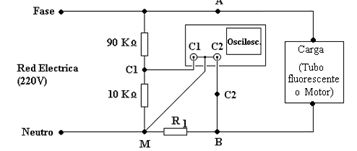
\includegraphics[width=0.7\linewidth]{Imagenes/exp1med.png}
    \caption{Circuito experimento 1}
    \label{fig:exp1med}
\end{figure}

Para poder calcular la potencia activa consumida por este circuito, es necesario a averiguar la corriente y la caída de tensión sobre el conjunto balastro/tubo fluorescente, además del factor de potencia.

Para medir estas magnitudes se debe usar el osciloscopio, con la precaución de que la tensión pico de la señal medida no sobre pase el limite de tensión soportado por el osciloscopio. 

Sabiendo que el valor eficaz nominal de la señal es de $V_{ef}=220V$ podemos calcular que la tensión pico de la señal es de $V_{p}=311V$, que es menor que la tensión soportada por el osciloscopio, la cual es $V_{max}=400V$. De todas maneras para asegurarnos la correcta y segura toma de las magnitudes, se colocó un divisor resistivo en paralelo al circuito que se quiere medir, de esta manera disminuyendo el valor de tensión en el punto $C1$. 

La corriente no se puede medir de forma directa en el osciloscopio, por lo tanto se colocó una resistencia en la misma rama del circuito de interés ($R1$), por lo que, midiendo el punto $C2$ se obtendrá la tensión producto de la corriente de la rama.

Además se debe determinar el factor de potencia. Considerando que la tensión y la corriente estaban originalmente en fase, el factor de potencia se transforma en un atraso de la corriente en comparación con la tensión:

\begin{equation}
    S=V_{cc}\cos{(w_ct)}\cdot I_{L} \cos{(w_ct+\phi)} \xrightarrow{\hspace{10pt}F\hspace{10pt}} S=V_{cc}\cdot I_{L} \cos{(\phi)}
\end{equation}

Este desfase, se podría obtener comparando las señales en el modo X-Y del osciloscopio:

\begin{figure}[H]
\centering
    \begin{minipage}{0.49\textwidth}
        \centering
        \begin{tikzpicture}[scale=0.6,every node/.style={transform shape}]
\def\scalTa{0.1};%EscalaTemporal señal 1
\def\scalTb{0.1};%EscalaTemporal señal 2
\def\scalVa{2};%EscalaVertical señal 1
\def\scalVb{2};%EscalaVertical señal 2
\def\offseta{0};%Nivel de offset de la señal señal 1
\def\offsetb{0};%Nivel de offset de la señal señal 2

%Lineas intermedias grilla
\foreach \x in {-5,-4.8,...,4.8,5}{
    \draw[gray!40,thin,shift={(\x,0)}] (0pt,2pt) -- (0pt,-2pt);
}
\foreach \y in {-4,-3.8,...,3.8,4}{
    \draw[gray!40,thin,shift={(0,\y)}] (2pt,0pt) -- (-2pt,0pt);
}
\foreach \a [evaluate={\y=\a*0.5}] in {-5,-1,1,5}{
    \draw[gray!40,line width=0.7pt,dotted] (-5,\y) -- (5,\y);
}

%Grilla
\draw[thin,gray!40] (-5,-4) grid (5,4);
\node[fill=white,text=gray!40,circle,scale=0.5] at (-5,3) {$100\%$};
\node[fill=white,text=gray!40,circle,scale=0.5] at (-5,2.5) {$90\%$};
\node[fill=white,text=gray!40,circle,scale=0.5] at (-5,-2.5) {$10\%$};
\node[fill=white,text=gray!40,circle,scale=0.5] at (-5,-3) {$0\%$};
\draw[black] (-6,-5) rectangle(6,5);

%Señal 1
\draw [mblk]plot[smooth,samples=100,domain=-5:5](\x,{\scalVa*(cos(deg(\x*pi*5*\scalTa))+\offseta)});
%Señal 2
\draw [mblk] plot[smooth,samples=100,domain=-5:5](\x,{\scalVb*(cos(deg(\x*pi*(5)*\scalTb+(pi/3)))+\offsetb)});

\end{tikzpicture}
\caption*{Compracion 2 señales}
    \end{minipage}
   \begin{minipage}{0.49\textwidth}
        \centering
        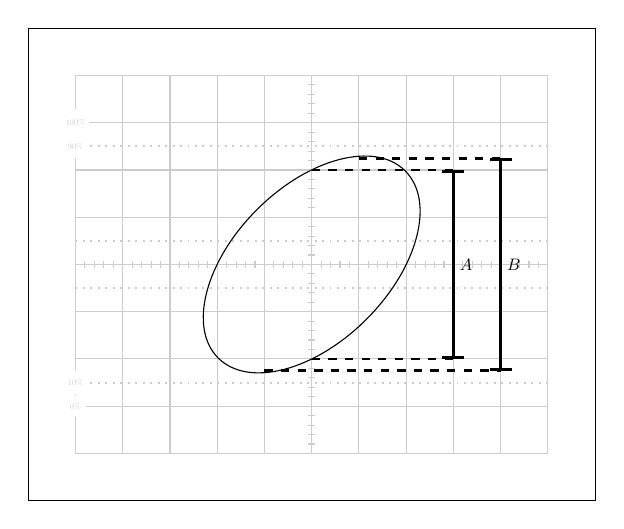
\begin{tikzpicture}[scale=0.6,every node/.style={transform shape}]
\def\scalTa{0.02};%EscalaTemporal señal 1
\def\scalTb{0.02};%EscalaTemporal señal 2
\def\scalVa{1};%EscalaVertical señal 1
\def\scalVb{1};%EscalaVertical señal 2
\def\offseta{0};%Nivel de offset de la señal señal 1
\def\offsetb{0};%Nivel de offset de la señal señal 2

%Lineas intermedias grilla
\foreach \x in {-5,-4.8,...,4.8,5}{
    \draw[gray!40,thin,shift={(\x,0)}] (0pt,2pt) -- (0pt,-2pt);
}
\foreach \y in {-4,-3.8,...,3.8,4}{
    \draw[gray!40,thin,shift={(0,\y)}] (2pt,0pt) -- (-2pt,0pt);
}
\foreach \a [evaluate={\y=\a*0.5}] in {-5,-1,1,5}{
    \draw[gray!40,line width=0.7pt,dotted] (-5,\y) -- (5,\y);
}

%Grilla
\draw[thin,gray!40] (-5,-4) grid (5,4);
\node[fill=white,text=gray!40,circle,scale=0.5] at (-5,3) {$100\%$};
\node[fill=white,text=gray!40,circle,scale=0.5] at (-5,2.5) {$90\%$};
\node[fill=white,text=gray!40,circle,scale=0.5] at (-5,-2.5) {$10\%$};
\node[fill=white,text=gray!40,circle,scale=0.5] at (-5,-3) {$0\%$};
\draw[black] (-6,-5) rectangle(6,5);

\draw[rotate=-45] (0, 0) ellipse (0.82cm*2 and 1.4cm*2);
\draw[line width=1pt,dashed](0,2)--(3,2);
\draw[line width=1pt,dashed](0,-2)--(3,-2);
\draw[line width=1pt,|-|](3,2)--(3,-2) node[midway,right]{$A$};
\draw[line width=1pt,dashed](1,2.25)--(4,2.25);
\draw[line width=1pt,dashed](-1,-2.25)--(4,-2.25);
\draw[line width=1pt,|-|](4,2.25)--(4,-2.25) node[midway,right]{$B$};
\end{tikzpicture}
\caption*{Modo X-Y}
    \end{minipage}
    \caption{}
    \label{fig:X-YeT}
\end{figure}

Y con estos datos ($A$ y $B$), se calcula el factor de potencia a través de la ecuación \ref{eq:Desf}:

\begin{equation}\label{eq:Desf}
    \cos{(\phi)}=\sqrt{1-(\frac{A}{B})} \hspace{5mm}\Longleftrightarrow\hspace{5mm} 
    \sin{(\phi)}=\frac{A}{B}
\end{equation}

\unsubsubsection{Mediciones}

Para calcular el factor de potencia se utilizó un osciloscopio de 2 canales, la punta del primer canal se colocó en el punto C1 midiendo así la forma y fase de la señal entrante de tensión. La segunda punta se colocó en el punto C2 midiendo el desfase de la tensión en $R1$ debido a la corriente $I_L$.

\begin{figure}[H]
    \begin{subfigure}{0.45\textwidth}
        \centering
        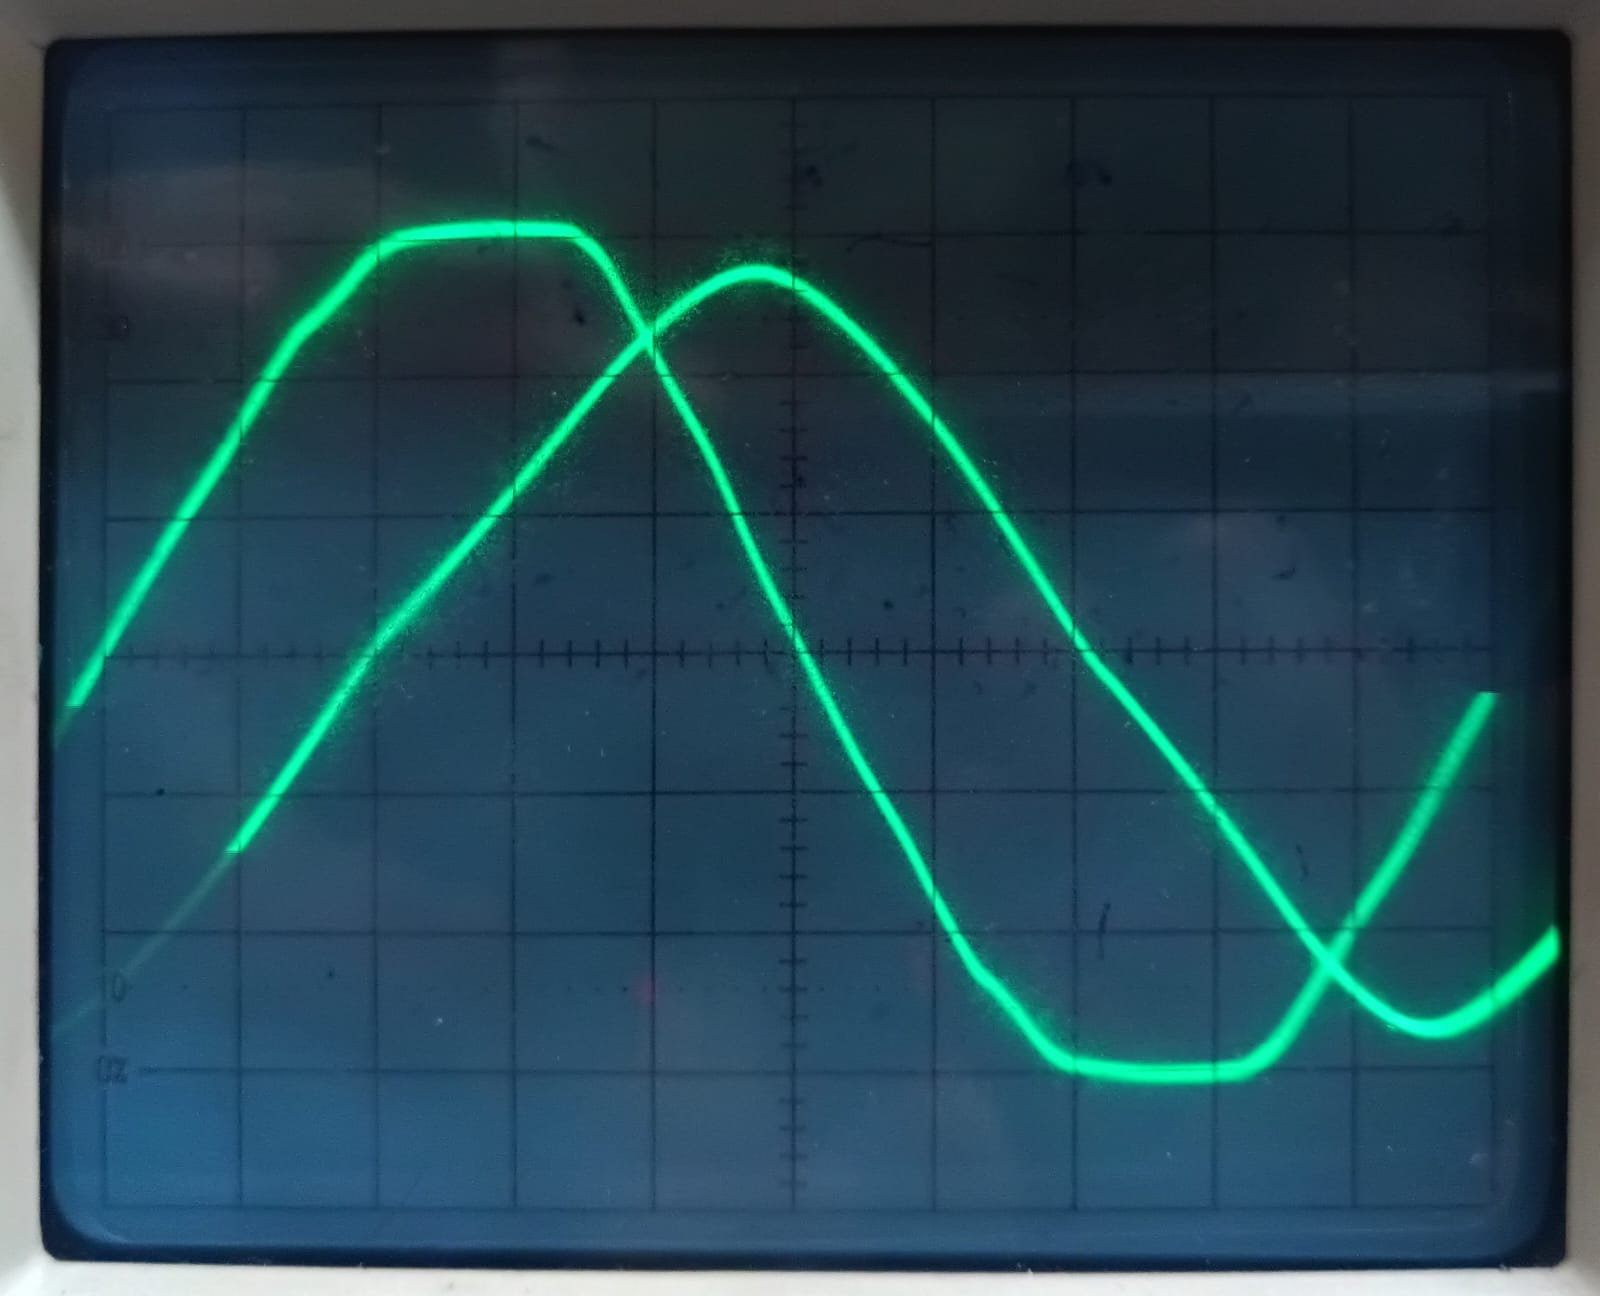
\includegraphics[width=1\linewidth]{Imagenes/Mediciones/desfExp1.jpeg}
        \caption{Señales desfasadas}
        \label{fig:desfExp1}
    \end{subfigure}
    \hspace*{\fill}
    \begin{subfigure}{0.45\textwidth}
        \centering
        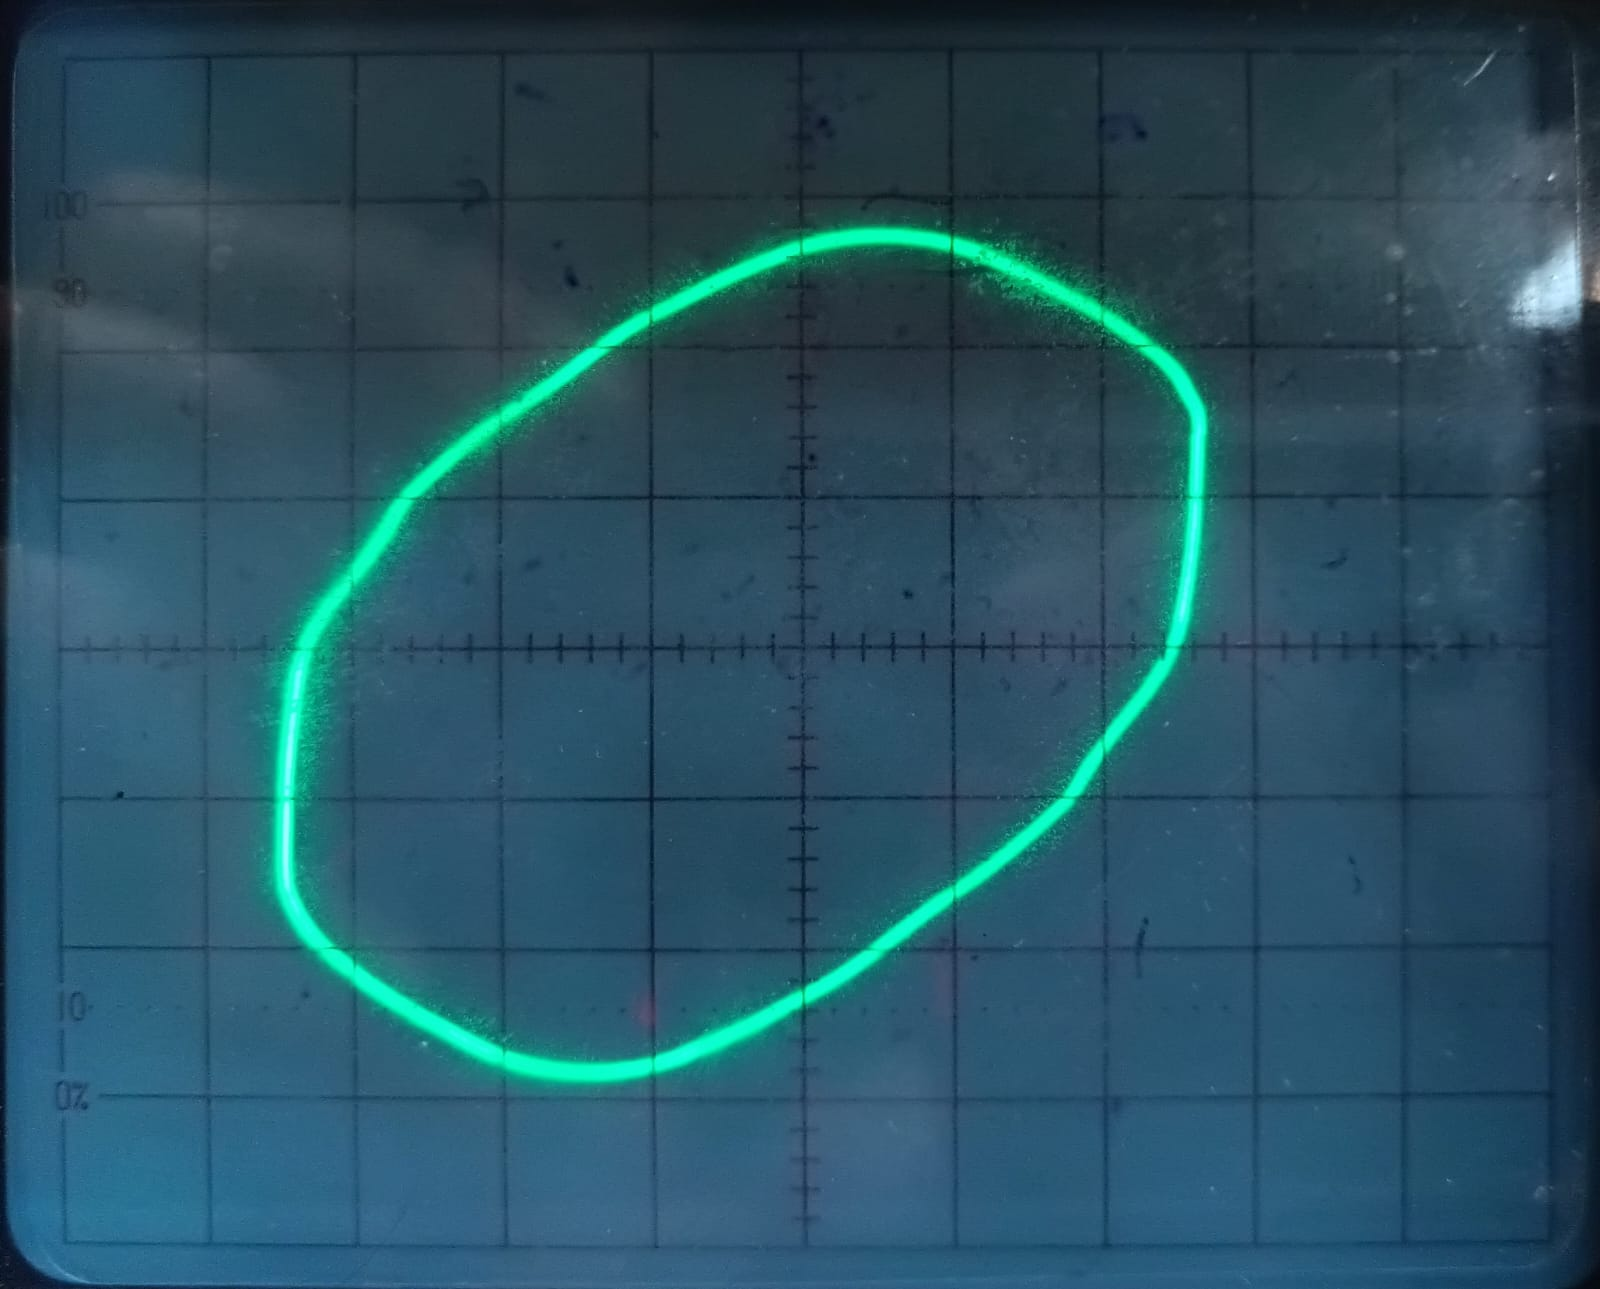
\includegraphics[width=1\linewidth]{Imagenes/Mediciones/lissajou.jpeg}
        \caption{Figura de Lissajou}
        \label{fig:corrFp}
    \end{subfigure}
\end{figure}

Para medir las amplitudes necesarias para la ecuación\ref{eq:Desf} se asociaron los valores del modo X-Y con las amplitudes de las señales de entrada, ($X$ siendo la señal 1 y la correspondiente en tiempo, e $Y$ la amplitud a medir). Para la amplitud A el valor de la componente $X$ es igual a cero entonces se midió la amplitud de la señal 2 en el momento en el cual la señal 1 tomaba amplitud 0 $A=9.8V$, de manera similar se determinó que el valor de la amplitud B es el valor máximo de la señal 2 $B=10.6V$.Utilizando la ecuación \ref{eq:Desf}:

\begin{equation*}
\begin{aligned}
     \cos{(\phi)}=&\sqrt{1-{\left(\frac{A}{B}\right)}^2}\\
                =&\sqrt{1-{\left(\frac{9.8}{10.6}\right)}^2}
                \\
                \cos{(\phi)}=&0.381\lrah\phi=67.6^\circ
\end{aligned}
\end{equation*}

Utilizando un multímetro \textit{TrueRMS} se observó que la corriente que alimenta a la lampara era de $I_{L}=365mA$, ya que la tensión sobre $R1=10\Omega$ era de $3,65V$. Observando la figura \ref{fig:desfExp1} podemos saber que la tensión sobre la lampara y el balastro va a ser la propia tensión de linea menos la caída de  sobre  la resistencia $R1$. Se midió que la tensión de linea era de aproximadamente $V_{cc}=233 V_{ef}$ y la caída de tensión en la resistencia, de $V_{R1}=3,65V$. Entonces la tensión que alimenta la rama estará dado por:

\begin{equation*}
\begin{aligned}
    V_{L}=V_{cc}\cdot\sqrt{2}\cdot\cos{(w_ct)}-I_L\cdot R_1\cos{(wc_t+\phi)}\xlongrightarrow{F}V_{Lef}&=233-3.65\cdot Arg(67.6)\\
    V_{Lef}&=233-(1.391+j3.375)\\
    V_{Lef}&=231.61-j3.375\\
    V_{Lef}&=231.61 Arg(0.317^\circ)
\end{aligned}
\end{equation*}
Se decidió no tener en cuenta el desfase de la tensión dado que era $0.00466$ veces el desfase correspondiente de la corriente.
Sabiendo estos datos se calculo que la potencia activa del circuito correspondiente a la rama de la lampara era de:
\begin{equation*}
    P_{activa}=231.61\cdot0.365\cdot\cos{(\phi)}\lrah P_{activa}=32.32 W
\end{equation*}
De manera similar se calcularon las potencias aparentes  y reactivas
\begin{equation*}
    Q_{reactiva}=231.61\cdot0.365\cdot\sin{(\phi)}=78.16
\end{equation*}
\begin{equation*}
    S_{aparente}=231.61\cdot0.365=84.54
\end{equation*}
%% hay que aclarar que las divisiones estaan en x10
\begin{table}[H]
    \centering
    \begin{tabular}{|c|c|c|c|c|c|}
    \hline
        & \multirow{2}{*}{V/div} & \multirow{2}{*}{$V_{pp}$} & $V_{ef}$  & $V_{ef}$ & Incertidumbre \\
        ~ &  &  & Osciloscopio & Mult. True RMS &  Multímetro \\ 
        \hline
        Canal 1 & 1 & 63.077 & V = 223.01   & V = 233 & $\pm$ 2.333 V\\ 
        \hline
        Canal 2 & 0.2 & 10.32 &  I  = 0.364mA   & I = 0.365mA & $\pm$ 0.01565 mA \\ 
        \hline
        \multicolumn{2}{|c|}{$\cos\phi=0.381$} & \multicolumn{2}{c|}{$sen\phi=0.925$} &
        \multicolumn{2}{c|}{$\tan\phi=2.426$}\\ 
        \hline
        \multicolumn{6}{|c|}{Potencia Activa: P = 32.32[W]}\\
        \hline
        \multicolumn{3}{|c|}{Pot. Reactiva: Q = 78.16[VAR]} & \multicolumn{3}{c|}{Pot. Aparente: S = 84.54[VA]}\\ \hline
    \end{tabular}
    \def\tablename{Tabla} 
    \caption{Tabla de mediciones del experimento 1}
    \label{tab:exp1}
\end{table}